\documentclass{article}

\usepackage{arxiv}
\usepackage[ruled,vlined]{algorithm2e}
\usepackage[utf8]{inputenc}
\usepackage[T1]{fontenc}
\usepackage{url}
\usepackage{booktabs}
\usepackage{amsfonts}
\usepackage{nicefrac}
\usepackage{microtype}
\usepackage{graphicx}
\usepackage[font=small,labelfont=bf]{caption}
\usepackage{cite}
\usepackage{pdflscape}
\usepackage{listings}
\usepackage{outlines}
\usepackage{tikz}
\usepackage{epigraph}
\usepackage{natbib} 
\usepackage{url}

\newcommand*\circled[1]{\tikz[baseline=(char.base)]{
		\node[shape=circle,draw,inner sep=1pt] (char) {#1};}}

\title{Preservation of log lineage under data tiering in Kafka}

\begin{document}
\maketitle \thispagestyle{fancy2}
\begin{abstract}
	The objective of this document is to elaborate on the design of a protocol which ensures the lineage of logs in Apache Kafka is preserved  when segments are moved to and accessed from external storage tier.
\end{abstract}

\section{Motivation}
\epigraph{\textit{"At its heart a Kafka partition is a replicated log"}}{Kafka online documentation \cite{RD1}}

As stated in the reference documentation and echoed in \cite{KDG}, replication in Apache Kafka is one of its most fundamental characteristic. The replication protocol which Kafka implements and the guarantees it provides are well documented \cite{KIP101} \cite{KIP279}, and explains how and why a consistent lineage for a topic-partition is preserved across its replicas irrespective of the nature and frequency of fail-overs that topic-partition experiences. 

One of the premise of the integration of data tiering in Apache Kafka is to provide users with a uniform experience of access to data irrespective of its provenance (the storage tier where it comes from). This especially means data lineage is kept consistent when tiered segments are the source of data and the specifications which apply to local replicas are still honored when tiered segments contribute to a replica's lineage.

This document assumes some level of familiarity with the replication protocol implemented in Kafka and how replica lineage is maintained across replicas. At a very high level, this protocol is based on \textit{log truncation}, which relies on replica history, materialized by a list of generation to start offset vectors, which evolves with cluster events and leadership migration. At a given point in time, the lineage of the log of a topic-partition is that of the leader replica of that topic-partition. It is possible for the end offset of the log to decrease when leadership is assigned to a different replica.

It also assumes familiarity with the design of tiered storage in Kafka, described in KIP-405 \cite{KIP405}.

\section{Replica lineage and tiered segments}

Consider a topic-partition with three replicas which experiences leadership migrations. The lineage tree of the topic-partition is provided below, along with the leadership assignments throughout the sequence of generations (leader epochs) of this topic-partition.

\subsubsection{Notations and simplifications}

\textbf{Serialized offsets}

We will informally select offsets from the available replicas at points of interest. An offset is written $\theta$ and indexed such that $\theta_{i+1}$ is written \textit{after} $\theta_i$ for any given index $i$. The use of generation makes this serialization possible. Note that $(\theta_i)_{i \in \mathbb{N}}$ is not necessarily monotonic.

\textbf{Generations}

A leader epoch is written $g$ and is indexed such that $g_{i+1}$ is younger than $g_i$. Note that, for simplicity, the exact sequence of incremental leader epochs is not reproduced. For instance, when replica 2 and 3 go offline in figure \ref{fig:lineage-tree-1}, leader epoch is expected to be incremented at least twice, but we will simply refer to the new leader epoch as $g_2$ even if it differs from $g_1$ by more than one increment.

\subsubsection{Lineage tree of the topic-partition}

Figure \ref{fig:lineage-tree-1} shows the content of the three replicas over generations depicted in figure \ref{fig:seq-generations}.

\begin{outline}[enumerate]
\1 The root of the tree corresponds to the subsegment of the range $[\theta_1, \theta_2]$, which is assumed to be common to all three replicas.
\1 At generation $g_2$, replicas 2 and 3 become offline and replica 1 ingest records from $\theta_{2} + 1$ to $\theta_3$. The segment with base offset $\theta_1$ and end offset $\theta_3$ is offloaded by replica 1\footnote{Here, the word \textit{replica} informally refers to the hosting \textit{broker}.}, with the leader epoch at the time of the offload, $g_2$.
\1 Replica 1 become offline and replica 2 and 3 now contribute to the ISR set. Replica 3 is the leader. The segment with the offset range $[\theta_1, \theta_4]$ is offloaded at generation $g_3$.
\1 Replica 2 falls behind and is moved out of ISR. Replica 3 continues to ingest and offload the segment ranging from offsets $[\theta_4 + 1, \theta_5]$ at generation $g_4$. This is possible because the ISR is reduced to its leader and the leader high watermark can freely moves forward.
\1 Leadership is transferred to replica 2 and replica 3 is put offline. The ISR set is now $\{2\}$. Data continues to be ingested.
\1 Replica 3 is back online. Generation is incremented to $g_6$ on this event. Truncation is performed, which physically deletes the segment $[\theta_{5}+1, \theta_{5}+2]$. The segment offloaded at generation $g_4$ is only in the external storage at truncation time. This segment is now \textit{orphan}, because no matter the following life events affecting the cluster, there is no going back and that part of the lineage is forever discarded. Another way to see it is that the edge from the prefix $[\theta_2+1,\theta_4]$ to $[\theta_4+1,\theta_6]$ in the lineage tree can be removed.
\1 The segment $[\theta_2+1,\theta_6]$ is rolled over and eventually become eligible for tiering. It is offloaded at generation $g_6$ by replica 2.
\end{outline}

The content of the tiered storage after these events is represented in figure \ref{fig:tiered-storage}.

\begin{figure}[h!]
	\centering
	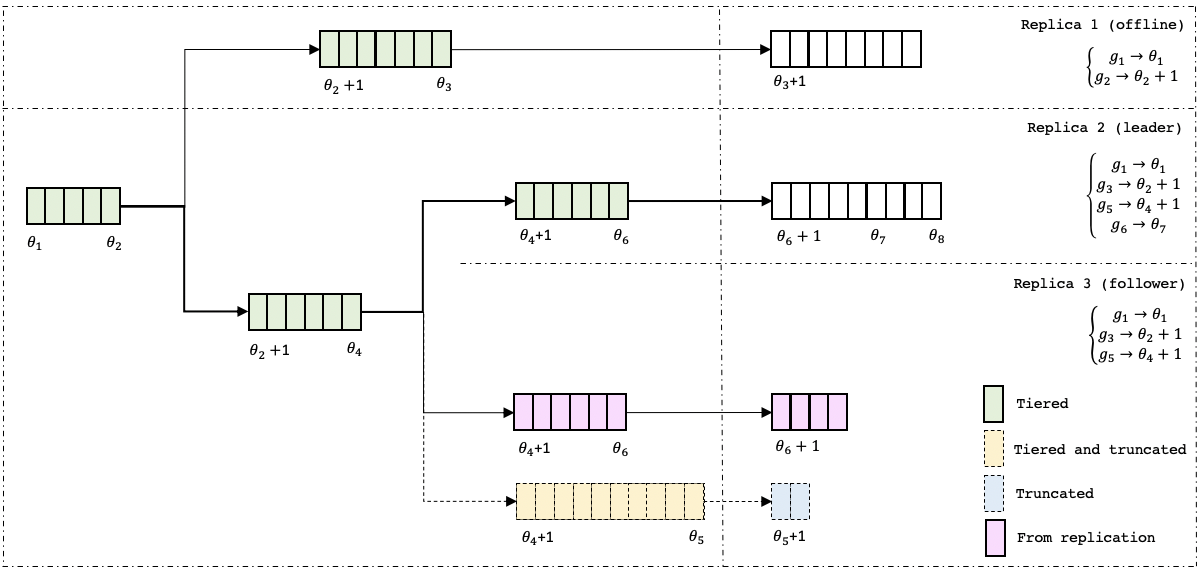
\includegraphics[scale=0.55]{lineage-tree-1.png}
	\captionof{figure}{Lineage tree of the topic-partition while replica 1 is offline. The generation-to-start-offset vectors, which build the leader epoch cache, are represented on the right.}
	\label{fig:lineage-tree-1}
\end{figure}

\begin{figure}[h!]
	\centering
	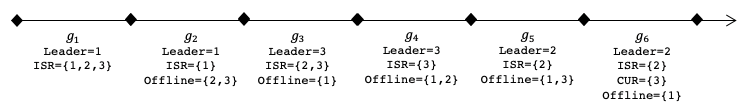
\includegraphics[scale=0.6]{seq-generations.png}
	\captionof{figure}{Lineage tree of the topic-partition while replica 1 is offline.}
	\label{fig:seq-generations}
\end{figure}

\begin{figure}[h!]
	\centering
	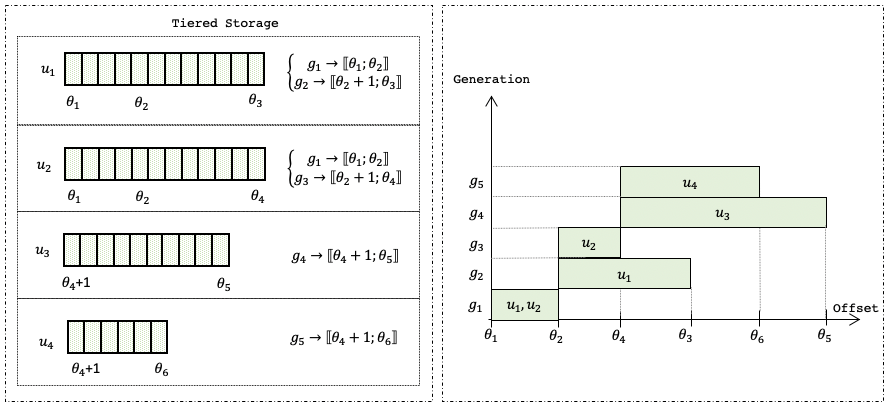
\includegraphics[scale=0.6]{tiered-storage.png}
	\captionof{figure}{Content of the tiered storage. Each segment is conceptually associated to a generation and a range of offsets which uniquely identify it in the history of the topic-partition across all replicas.}
	\label{fig:tiered-storage}
\end{figure}

\subsubsection{Tiering reconcilation on become-leader}

A replica which becomes the leader of a topic-partition, and detects tiered segments for that topic-partition, tries to identify which parts of its lineage are present in the tiered storage. This allows the leader a) to know which of the local segments need to be offloaded, if any, b) to know what is the largest offset in tiered segments which is part of its lineage.

Looking back at the previous example, if a replica happened to become the leader of the topic-partition, it would use its local epoch cache and the history of lineage of this topic-partition covered in the tiered storage, represented as a graph $\mathcal{G}=(\theta,g)$ which provides the ranges of offsets of the tiered segments along with the epoch of the leader which offloaded them.



guarantee the following property: for any given offset in a segment of the leader replica which is present in the tiered storage, prior offsets which make up the contemporary\footnote{i.e. excluding segments evicted from the local and/or tiered storage} lineage of the leader replica are also present in the tiered storage. Informally, that means there is no "gap" in the range of offsets which are present in the tiered storage, without a segment which would only be available locally between two tiered segments.

\subsubsection{Remote end offset resolution on become-follower}

When replica 1 becomes online and initiates replication from replica 2, it needs to know:

\begin{outline}[enumerate]
\1 Its truncation and fetch offset, this is implemented with the truncation protocol;
\1 The range of offsets which is already tiered, and which should not be replicated from the leader.
\end{outline}


All the follower need to know is the last offset of the latest tiered segment according to the current replica lineage. In the case of the lineage tree in figure \ref{fig:lineage-tree-1}, that would be $\theta_6$. Note that this is not necessarily the \textit{latest} segment offloaded, nor the largest offset of all the segments offloaded for that topic-partition ($\theta_6 < \theta_5$).





fd

\newpage
\bibliographystyle{plain}
\bibliography{tiered-storage-replication}{}
\end{document}
